\documentclass[margin=1em]{standalone}

\usepackage{pgfplots}
\pgfplotsset{compat=1.10}   % in my packages used compat=1.15
\usepgfplotslibrary{fillbetween}
\usepackage{pgf}
\usepackage{tikz}
\usetikzlibrary{patterns,arrows,calc,decorations.pathmorphing,backgrounds, positioning,fit,petri,decorations.fractals}
\usetikzlibrary{matrix}

\usepackage[table,dvipsnames]{tudscrcolor}

\usepackage[default]{opensans}

\begin{document}
	\color{cddarkblue}
	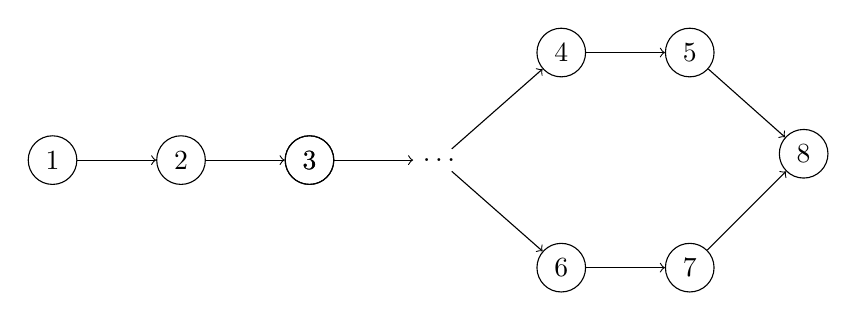
\begin{tikzpicture}[]
		\node [circle,draw] (1) {$1$};
		\node [circle,draw,right=of 1] (2) {$2$};
		\node [circle,draw,right=of 2] (3) {$3$};
		\node [circle,draw,right=of 2] (3) {$3$};
		\node [right=of 3] (dots) {$\dots$};
		\node [circle,draw,above right=of dots] (4) {$4$};
		\node [circle,draw,right=of 4] (5) {$5$};
		\node [circle,draw,below right=of dots] (6) {$6$};
		\node [circle,draw,right=of 6] (7) {$7$};
		\node [circle,draw,above right=of 7] (8) {$8$};
		
		% Kanten
		% \path (1) -> node[weight] {$3$} (3)
		\draw[->] (1) -> (2);
		\draw[->] (2) -> (3);
		\draw[->] (3) -> (dots);
		\draw[->] (dots) -> (4);
		\draw[->] (4) -> (5);
		\draw[->] (5) -> (8);
		\draw[->] (dots) -> (6);
		\draw[->] (6) -> (7);
		\draw[->] (7) -> (8);
	\end{tikzpicture}
\end{document}